% !TeX program = pdflatex
%==============================================================================
%  Aula E2 --- Redução de Dimensionalidade (PCA e t-SNE)
%  VERSÃO DO ALUNO: texto para leitura autônoma, fora da sala.
%  (O roteiro de sala é "E2 Reducao de Dimensionalidade PCA e t-SNE.tex".)
%==============================================================================
\documentclass[11pt,a4paper]{article}
\usepackage[aluno]{../../recursos/latex/estilo-notas}

\title{}
\date{}

\begin{document}
\cabecalhoaula{Extra E2}{Redução de Dimensionalidade (PCA e t-SNE)}{AME cap.~10; ISLP §12.2}

%==============================================================================
\section*{O que você vai aprender}
%==============================================================================
Ao final desta aula você deve ser capaz de:
\begin{itemize}[leftmargin=1.4cm]
  \item listar as razões para reduzir a dimensionalidade;
  \item definir os \textbf{componentes principais} como direções de variância
        máxima e resolvê-los via autovetores;
  \item usar a \emph{proporção de variância explicada} para escolher quantos
        componentes manter;
  \item interpretar o PCA geometricamente e usá-lo para \textbf{compressão};
  \item reconhecer as extensões não lineares --- \textbf{Kernel PCA} e
        \textbf{t-SNE} --- e os cuidados com este último.
\end{itemize}

\noindent
Esta aula ataca de frente a maldição da dimensionalidade da Aula~05, mas pelo lado
da \emph{redundância}: se as covariáveis são correlacionadas, os dados ocupam
apenas uma fatia fina do espaço $\R^p$, e talvez baste descrevê-la. A pergunta:

\begin{center}\itshape
  como resumir $p$ covariáveis em bem menos, sem perder o essencial?
\end{center}

%==============================================================================
\section{Por que reduzir a dimensionalidade?}
%==============================================================================
\begin{itemize}[leftmargin=1.4cm,nosep]
  \item \textbf{Visualização}: projetar dados em 2D/3D para enxergar estrutura.
  \item \textbf{Compressão}: armazenar/transmitir com menos espaço (imagens).
  \item \textbf{Pré-processamento}: combater a \emph{maldição da dimensionalidade}
        (Aula~05) e o ruído antes de um método supervisionado.
  \item \textbf{Redundância}: muitas covariáveis correlacionadas vivem perto de uma
        subvariedade de dimensão menor --- queremos recuperá-la.
\end{itemize}

\begin{ideia}
O último item é o mais importante conceitualmente, e liga esta aula ao Bloco~I. Na
Aula~05 vimos que o KNN \emph{se adapta sozinho} à dimensão
intrínseca $u$, mas que métodos que somam todas as coordenadas sofrem com $p$
grande. O PCA faz esse trabalho \emph{explicitamente}: ele encontra a subvariedade
--- desde que ela seja aproximadamente um subespaço linear.
\end{ideia}

%==============================================================================
\section{Componentes principais (PCA)}
%==============================================================================
Suponha as covariáveis \emph{centradas} (média zero). O \textbf{primeiro componente
principal} é a combinação linear
\[
  Z_1 = \phi_{11}X_1+\dots+\phi_{p1}X_p = \bm{\phi}_1^\top\X
\]
de \textbf{variância máxima}, sob a restrição $\norm{\bm{\phi}_1}^2=\sum_k\phi_{k1}^2=1$
(sem ela, bastaria inflar os coeficientes). O $i$-ésimo componente $Z_i$ tem variância
máxima entre as combinações lineares unitárias \emph{não correlacionadas} com
$Z_1,\dots,Z_{i-1}$.

\begin{ideia}
Procuramos novos eixos (ortogonais) ao longo dos quais os dados \emph{mais variam}.
O 1º eixo capta o máximo de variabilidade; o 2º, o máximo do que resta sendo
ortogonal ao 1º; e assim por diante. Concentrar a variância em poucos eixos é o que
permite descartar os demais com pouca perda.
\end{ideia}

\begin{figure}[htbp]
  \centering
  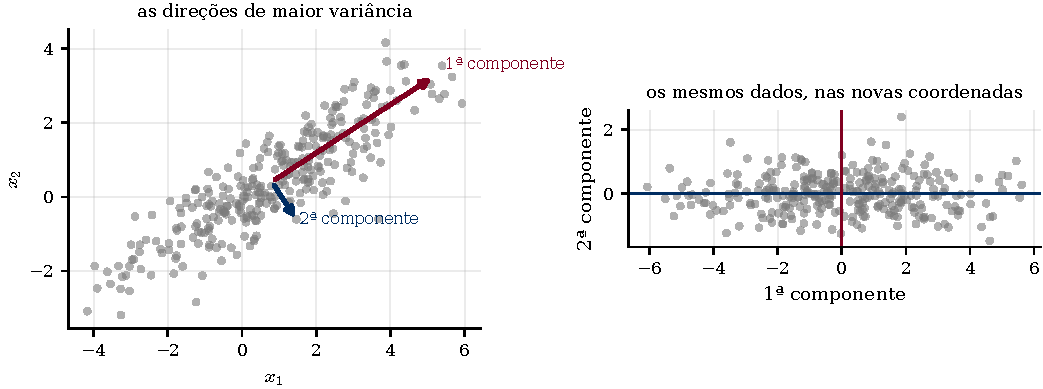
\includegraphics[width=\textwidth]{../../recursos/figuras/E2-eixos.pdf}
  \caption{PCA em duas dimensões. À esquerda, a nuvem original e as duas direções
  principais, com comprimento proporcional ao desvio-padrão ao longo delas: a
  primeira acompanha o alongamento da nuvem e responde por $94{,}4\%$ da variância.
  À direita, os mesmos pontos escritos nas novas coordenadas --- é literalmente uma
  \emph{rotação}. E é aí que a redução fica óbvia: descartar a segunda coordenada
  custa $5{,}6\%$ da variância e transforma dois números em um.}
  \label{fig:eixos}
\end{figure}

\subsection{Solução: autovetores da covariância}
Seja $\bm{C}=\bm{X}^\top\bm{X}$ (proporcional à matriz de covariância, pois os dados
têm média zero). O problema é
\[
  \max_{\bm{\phi}}\ \Var(\bm{\phi}^\top\X) = \max_{\bm{\phi}}\ \bm{\phi}^\top\bm{C}\bm{\phi}
  \quad\text{s.a.}\quad \norm{\bm{\phi}}^2=1.
\]

\begin{proposicao}[O 1º componente é o autovetor principal]\label{prop:pca}
O maximizador de $\bm{\phi}^\top\bm{C}\bm{\phi}$ sob $\norm{\bm{\phi}}=1$ é o
autovetor de $\bm{C}$ associado ao \emph{maior} autovalor, e o valor máximo da
variância é esse autovalor.
\end{proposicao}
\begin{proof}
Lagrangiano: $\mathcal{L}(\bm{\phi},\nu)=\bm{\phi}^\top\bm{C}\bm{\phi}
-\nu(\bm{\phi}^\top\bm{\phi}-1)$. Anulando o gradiente em $\bm{\phi}$:
$2\bm{C}\bm{\phi}-2\nu\bm{\phi}=0$, isto é, $\bm{C}\bm{\phi}=\nu\bm{\phi}$ ---
$\bm{\phi}$ é \emph{autovetor} de $\bm{C}$ com autovalor $\nu$. Para um autovetor
unitário, a variância é $\bm{\phi}^\top\bm{C}\bm{\phi}=\nu$. Logo o máximo é atingido
no autovetor de \emph{maior} autovalor. Os componentes seguintes saem do mesmo
argumento restrito ao complemento ortogonal, gerando os demais autovetores em ordem
decrescente de autovalor.
\end{proof}

\begin{ideia}
Vale apreciar quanto essa proposição entrega. O problema original --- ``ache a
melhor direção, depois a melhor entre as ortogonais a ela, e assim por diante''
--- parece uma sequência de $p$ otimizações encadeadas. A proposição diz que
\textbf{uma única} decomposição espectral de $\bm{C}$ resolve todas de uma vez, e
ainda ordena o resultado. É por isso que o PCA é barato mesmo com $p$ grande.
\end{ideia}

Empilhando os autovetores (ordenados por autovalor decrescente) nas colunas de
$\bm{U}$ (a \textbf{matriz de cargas}), os \emph{scores} são
\[
  \bm{Z} = \bm{X}\bm{U}\quad (n\times p),
\]
e a $i$-ésima nova coordenada da observação $\x$ é $z_{i}=\bm{u}_i^\top\x$. Como os
autovetores são ortogonais, os componentes são \emph{não correlacionados} --- sem
informação redundante.

\subsection{Quantos componentes? Variância explicada}
Cada autovalor $\lambda_i$ é a variância capturada pelo $i$-ésimo componente. A
\textbf{proporção de variância explicada} pelos $p$ primeiros é
\begin{equation}\label{eq:pve}
  \text{PVE}(p) = \frac{\sum_{i=1}^p \lambda_i}{\sum_{i=1}^p \lambda_i}.
\end{equation}
Escolhe-se $p$ olhando o \emph{scree plot} ($\lambda_i$ vs.\ $i$, procurando o
``cotovelo'') ou exigindo PVE acima de um limiar (ex.: 90\%).

\begin{figure}[htbp]
  \centering
  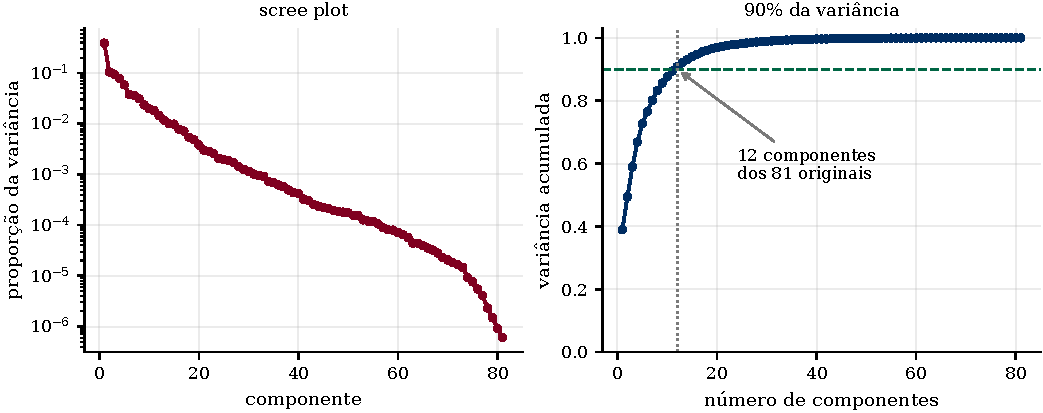
\includegraphics[width=\textwidth]{../../recursos/figuras/E2-variancia.pdf}
  \caption{PCA nas $81$ covariáveis padronizadas do \texttt{superconductivity.csv},
  a mesma base das aulas práticas. O primeiro componente sozinho explica $38{,}9\%$
  da variância, e \textbf{12 componentes} chegam a $90\%$. Em outras palavras: as
  $81$ colunas carregam cerca de uma dúzia de dimensões de informação, e as demais
  $69$ são, em boa medida, repetição. É a \emph{redundância} da Aula~05, medida.}
  \label{fig:variancia}
\end{figure}

%==============================================================================
\section{Interpretação geométrica e compressão}
%==============================================================================
\subsection{PCA como escalonamento multidimensional}
O PCA também resolve: encontrar a projeção linear $\bm{Z}$ em $m<p$ dimensões que
melhor \emph{preserva as distâncias} entre pares,
\[
  \min_{\bm{Z}}\ \sum_{i,j}\big(\norm{\x_i-\x_j}^2 - \norm{\bm{z}_i-\bm{z}_j}^2\big).
\]
A solução são os $m$ primeiros componentes principais. Ou seja, PCA é a melhor
aproximação linear de baixa dimensão no sentido de distâncias --- daí ser tão útil
para visualização. Note que são \emph{dois} problemas aparentemente diferentes
(maximizar variância, preservar distâncias) com a \emph{mesma} solução; guarde isso,
porque o t-SNE vai atacar o segundo problema por outro caminho.

\subsection{Compressão (SVD truncada)}
Da decomposição $\bm{X}^\top\bm{X}=\bm{U}\bm{\Sigma}\bm{U}^\top$, reconstrói-se
$\bm{X}\approx \bm{Z}_p\bm{U}_p^\top$, usando só as $p$ primeiras colunas. Se os
autovalores decaem rápido, a reconstrução é quase perfeita guardando apenas
$(z_{i,1},\dots,z_{i,p})$ e as $p$ cargas $\bm{u}_1,\dots,\bm{u}_p$ --- uma
\textbf{compressão}.

\begin{figure}[htbp]
  \centering
  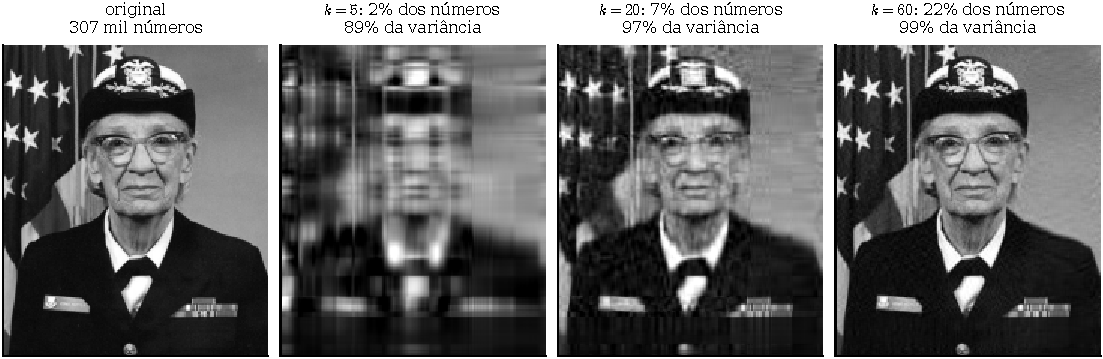
\includegraphics[width=\textwidth]{../../recursos/figuras/E2-compressao.pdf}
  \caption{Uma imagem em tons de cinza $600\times512$ ($307$ mil números) reconstruída
  a partir de $k$ componentes. Com $k=5$ guardamos $2\%$ dos números e já temos
  $89\%$ da variância --- e a imagem, embora borrada, tem a silhueta certa. Com
  $k=20$ ($7\%$ dos números) o rosto é reconhecível; com $k=60$ ($22\%$), a
  diferença para o original quase não se vê. A queda rápida dos autovalores é a
  razão de tudo isso funcionar.}
  \label{fig:compressao}
\end{figure}

\begin{atencao}
PCA usa variância e produtos internos $\Rightarrow$ é \textbf{sensível à escala}.
\emph{Padronize} as covariáveis antes (Aula~07), senão variáveis de maior magnitude
dominam os componentes artificialmente --- trocar metros por milímetros numa coluna
muda o resultado. E PCA é \emph{não supervisionado}: a direção de maior variância
\emph{não} é necessariamente a mais útil para prever um $Y$. É perfeitamente
possível que o sinal preditivo esteja justamente no componente de menor variância,
que você acabou de descartar.
\end{atencao}

%==============================================================================
\section{Além do linear: Kernel PCA e t-SNE}
%==============================================================================
\subsection{Kernel PCA}
PCA só captura estrutura \emph{linear}. Como o PCA pode ser escrito em termos de
produtos internos, aplica-se o \textbf{truque do \emph{kernel}} (Aulas~04 e~10):
substituem-se os produtos internos por um kernel $K$, fazendo PCA num espaço de
\emph{features} de alta dimensão. Resultado: componentes \textbf{não lineares}, que
capturam subvariedades curvas. É literalmente o mesmo truque da Aula~10, aplicado a
outro problema --- e essa recorrência não é coincidência: qualquer método que só
dependa de produtos internos admite a mesma generalização.

\subsection{t-SNE}
O \textbf{t-SNE} (\emph{t-distributed Stochastic Neighbor Embedding}) é uma técnica
\emph{não linear} feita para \textbf{visualização} (2D/3D). A ideia:
\begin{itemize}[leftmargin=1.4cm,nosep]
  \item converte distâncias em \textbf{probabilidades de vizinhança} no espaço
        original (kernel gaussiano) e no espaço reduzido (distribuição $t$ de
        Student, de caudas pesadas);
  \item ajusta as posições no espaço reduzido minimizando a divergência de
        \textbf{Kullback--Leibler} entre as duas distribuições;
  \item assim, \emph{preserva a estrutura local} (vizinhos próximos continuam
        próximos), revelando agrupamentos.
\end{itemize}
O principal hiperparâmetro é a \textbf{perplexidade} (ordem de grandeza do número de
vizinhos considerados).

\begin{ideia}[por que a distribuição $t$]
O detalhe do nome tem uma razão precisa. Ao espremer dados de $\R^p$ em $\R^2$, não
há espaço para manter todo mundo afastado --- pontos moderadamente distantes seriam
esmagados uns sobre os outros. A distribuição $t$, com caudas pesadas, atribui
probabilidade razoável a distâncias grandes no espaço reduzido, o que permite ao
algoritmo \emph{espalhar} os grupos em vez de amontoá-los. É uma solução para um
problema de espaço, não de estatística.
\end{ideia}

\begin{atencao}[Cuidados com o t-SNE]
\begin{itemize}[leftmargin=1.2cm,nosep]
  \item é \textbf{só para visualização} --- não use os eixos como \emph{features}
        para um modelo supervisionado (e note que, ao contrário do PCA, ele nem tem
        um \texttt{transform} para aplicar a dados novos);
  \item \textbf{distâncias e tamanhos} entre grupos no gráfico \emph{não} têm
        significado --- só a vizinhança local é confiável. Dois grupos afastados na
        figura não são necessariamente mais diferentes que dois próximos;
  \item é \textbf{estocástico} e sensível à perplexidade: rode mais de uma vez e
        compare. Se os agrupamentos mudam de uma rodada para outra, eles não estão
        nos dados. Para grandes bases, UMAP é uma alternativa mais rápida.
\end{itemize}
\end{atencao}

\noindent Em resumo: PCA para \emph{compressão e pré-processamento} (linear,
interpretável, com \texttt{transform} aplicável a dados novos); t-SNE para
\emph{olhar} os dados, e só.

%==============================================================================
\section{Prática em Python}
%==============================================================================
\begin{lstlisting}
from sklearn.decomposition import PCA
from sklearn.manifold import TSNE
from sklearn.preprocessing import StandardScaler
from sklearn.pipeline import make_pipeline

# PCA como etapa de um pipeline (Aula 07): ajustado SO no treino
pipe = make_pipeline(StandardScaler(), PCA(n_components=0.90), Ridge())

# quanta variancia cada componente explica
pca = PCA().fit(StandardScaler().fit_transform(X))
print(pca.explained_variance_ratio_.cumsum())

# t-SNE: apenas para visualizar. O init explicito importa -- com "pca" o
# resultado e reprodutivel; com "random", cada semente da outra figura
Z = TSNE(n_components=2, perplexity=30, init="pca",
         random_state=0).fit_transform(X)
\end{lstlisting}
O truque do \texttt{n\_components=0.90} é útil: em vez de um número de componentes,
passa-se a \emph{proporção de variância} desejada, e o \texttt{scikit-learn} escolhe
$p$ sozinho.

\begin{atencao}[qual é, afinal, a gravidade desse vazamento]
O PCA aprende direções a partir dos dados, então pela regra da Aula~07 ele é etapa
do modelo e tem de entrar no \emph{pipeline}. Mas vale ser preciso sobre a
\emph{gravidade}, porque a intuição engana aqui.

O que torna grave o vazamento por seleção de variáveis (Aula~07) é que a seleção
\textbf{olha o $Y$}: ela escolhe as colunas que, por acaso, se parecem com a
resposta naquela amostra, e é assim que fabrica $R^2=0{,}40$ a partir de ruído puro.
O PCA \textbf{não olha o $Y$}. Sem a resposta, não há como escolher direções que
finjam explicar ruído.

E a medição confirma: o notebook desta aula repete o experimento cruel da Aula~07 --
$y$ de ruído puro -- em quatro configurações de $(n,p,k)$, e em \emph{nenhuma} delas
calcular o PCA fora da dobra inflou o $R^2$. Ele o \emph{piorou}, porque componentes
calculados sobre o conjunto todo não são os componentes ótimos de nenhuma dobra de
treino. Na hierarquia da Aula~07, portanto, o PCA fica na categoria \textbf{leve},
ao lado da padronização --- e a conduta continua a mesma, porque corrigir custa uma
linha.
\end{atencao}

Os notebooks \texttt{Aula prática E2} e \texttt{Exemplo - PCA} ilustram os
componentes principais e a variância
explicada em dados reais.

%==============================================================================
\section*{Resumo}
%==============================================================================
\begin{itemize}[leftmargin=1.4cm]
  \item Reduzir dimensão serve para visualizar, comprimir, pré-processar e explorar
        \emph{redundância} (Aula~05).
  \item \textbf{PCA}: direções ortogonais de variância máxima; são os autovetores de
        $\bm{X}^\top\bm{X}$ em ordem de autovalor (Prop.~\ref{prop:pca}), obtidos de
        uma única decomposição (Fig.~\ref{fig:eixos}).
  \item \emph{Proporção de variância explicada} \eqref{eq:pve} guia a escolha de
        $p$: no \texttt{superconductivity}, 12 dos 81 componentes dão 90\%
        (Fig.~\ref{fig:variancia}).
  \item PCA $=$ melhor projeção linear no sentido de distâncias; a truncagem da SVD
        é compressão (Fig.~\ref{fig:compressao}).
  \item \emph{Padronize} antes; e lembre que PCA é não supervisionado --- a direção
        de maior variância pode não ser a mais preditiva.
  \item \textbf{Kernel PCA} e \textbf{t-SNE} estendem para o não linear; o t-SNE é
        \emph{só} para visualização, e distâncias entre grupos nele não significam
        nada.
\end{itemize}

\paragraph{Leitura recomendada.} [AME] Capítulo~10: §10.1 (PCA e a interpretação
como escalonamento multidimensional), §10.1.2 (compressão de imagens, que é a nossa
Figura~\ref{fig:compressao}), §10.2 (Kernel PCA) e §10.4 (\emph{autoencoders}, a
generalização não linear via redes neurais). [ISLP] §12.2 --- §12.2.1--12.2.2 (o que
são os componentes e a interpretação alternativa), §12.2.3 (proporção de variância
explicada, a nossa Figura~\ref{fig:variancia}) e §12.2.4, que discute honestamente
quantos componentes usar e por que não há resposta objetiva.

\paragraph{Para praticar.} \texttt{Lista teorica E2.pdf} (teórica, com gabarito) e \texttt{Lista prática E2.ipynb} (prática, para completar as lacunas), nesta mesma pasta.

\end{document}
